\documentclass[10pt]{article}

\usepackage[margin=0.78in]{geometry}
\usepackage{amsmath,amssymb,bm}
\usepackage{booktabs}
\usepackage{graphicx}
\usepackage{tabularx}
\usepackage{xcolor}
\usepackage{microtype}
\usepackage[hidelinks]{hyperref}
\hypersetup{
  pdftitle={Prism--Eta2: Formulation, Contribution Boundary, and Measured Bundle-Adjustment Performance},
  pdfauthor={Prism BA Research Project}
}

\graphicspath{{figures/convergence/}}
\setlength{\parindent}{0pt}
\setlength{\parskip}{0.55em}
\setlength{\tabcolsep}{4.5pt}
\renewcommand{\arraystretch}{1.12}

\newcommand{\R}{\mathbb{R}}
\newcommand{\F}{\mathcal{F}}
\newcommand{\Oset}{\mathcal{O}}
\newcommand{\EtaTwo}{Eta2}
\newcommand{\method}{Prism--Eta2}
\newcommand{\targettime}{time-to-target}
\newcolumntype{L}[1]{>{\raggedright\arraybackslash}p{#1}}
\newcolumntype{Y}{>{\raggedright\arraybackslash}X}

\title{\vspace{-1.5em}\textbf{Prism--Eta2: Formulation, Contribution Boundary, and Measured Bundle-Adjustment Performance}}
\author{Prism BA Research Project\\\small Technical report for internal review}
\date{13 September 2026}

\begin{document}
\maketitle

\begin{abstract}
This report describes the frozen Eta2 configuration of Prism, a GPU bundle-adjustment solver built around radius-controlled inexact Levenberg--Marquardt, matrix-free Schur elimination, camera-block preconditioned conjugate gradients, nonlinear point safeguards, and persistent recovery from numerical Schur-curvature failures.  We give the objective, damped block system, reduced camera equations, forcing rule, radius and acceptance policy, and the exact separability statement behind the point safeguard.  We then distinguish standard ingredients from the contributions that the present evidence can support.  The strongest claim is a numerical-optimization and systems result rather than a new trust-region theorem: the integrated solver reaches fixed, independently audited quality targets rapidly, while a large ablation campaign exposes when improvements to the linear algebra do not improve the nonlinear trajectory.  On the largest BAL instance tested, with 13,682 cameras and 28,987,644 observations, frozen Eta2 reaches the registered target in a median 3.239 seconds, versus 7.084 seconds for the measured Caspar FP32 configuration and 14.973 seconds for Caspar FP64.  On a separate three-instance, nine-target panel, Eta2 is fastest among all measured Prism, Caspar, and CPU Ceres configurations in all nine cells.  These results support a fastest-among-tested statement under the frozen protocol; they do not establish a universal fastest bundle-adjuster claim.
\end{abstract}

\section{Scope and configuration identity}

The subject of this report is the \emph{frozen Eta2 scientific champion}, not every experimental path in the Prism repository.  The measured configuration is pinned by \texttt{champion.json}, its source and headers by \texttt{source\_manifest.json}, and its binary by SHA-256.  It uses one damping candidate (\texttt{OCA\_NSHIFTS=1}) and does not use a multi-shift candidate menu, a learned policy, periodic retriangulation, or cross-iteration Krylov reuse.  The name Eta2 denotes a fixed modification of the inexact-solve forcing tolerance; it is not an RL agent and it does not set a tolerance equal to 2.

There is also a later, separately named systems build, B6v7.  It preserves the frozen mathematical method while changing reductions and preparation work.  We report its result separately in Section~\ref{sec:b6v7}; results attributed to the scientific champion remain those of the pinned Eta2 binary.

\section{Bundle-adjustment formulation}

\subsection{State, projection, and objective}

Let camera $i$ have rotation $R_i\in\mathrm{SO}(3)$, translation $t_i\in\R^3$, focal length $f_i$, and one active radial-distortion coefficient $k_i$.  The implementation retains the nine-parameter BAL storage convention but fixes the second radial coefficient to zero.  Let $X_j\in\R^3$ be landmark $j$, and let $x_{ij}\in\R^2$ be its measured image location in camera $i$.  With
\[
  Y_{ij}=R_iX_j+t_i,\qquad
  q_{ij}=\frac{(Y_{ij,1},Y_{ij,2})^T}{Y_{ij,3}},
\]
write the SIMPLE\_RADIAL projection compactly as
\[
  \pi(c_i,X_j)=f_i\bigl(1+k_i\lVert q_{ij}\rVert^2\bigr)q_{ij},
\]
up to the fixed BAL image-axis sign convention used consistently by the loader and evaluator.  The residual and scored objective are
\begin{align}
  r_{ij}(c_i,X_j)&=\pi(c_i,X_j)-x_{ij},\\
  F(c,X)&=\frac12\sum_{(i,j)\in\Oset}\lVert r_{ij}(c_i,X_j)\rVert^2. \label{eq:objective}
\end{align}
All reported methods are scored on the same original observations and the same plain $L_2$ objective in Eq.~\eqref{eq:objective}.  Intrinsics are unshared, $k_2$ is fixed to zero, and no robust loss or observation deletion is hidden in the score.  Camera rotations use the code's local retraction; point updates are additive.

The objective has the usual seven-dimensional similarity gauge\cite{Triggs2000}.  More consequential in the measured tail cases is the projective denominator $Y_{ij,3}$: a tiny change in state near $Y_{ij,3}=0$ can cause a large nonlinear change that a local quadratic model does not predict well.

\subsection{Linearization and damped normal equations}

Stack the camera and point increments as $d=(d_c,d_p)$ and linearize
\[
  r(x\oplus d)\approx r(x)+J_cd_c+J_pd_p,
\]
where $\oplus$ applies the camera retraction and additive point update.  Define
\[
  U=J_c^TJ_c+Q_{\mathrm{intr}},\qquad
  V=J_p^TJ_p,\qquad
  W=J_c^TJ_p,
\]
and $g_c=J_c^Tr$, $g_p=J_p^Tr$.  The nonnegative diagonal $Q_{\mathrm{intr}}$ stabilizes the linear solve and is excluded from the scored objective.  Each residual touches one camera and one point, so $U$ is camera-block diagonal before elimination and $V$ is point-block diagonal with $3\times3$ blocks.

For camera damping $\lambda$ and point damping $\tau$, the ideal damped Gauss--Newton equations are
\begin{equation}
\begin{bmatrix}
U+\lambda D_c & W\\
W^T & V+\tau D_p
\end{bmatrix}
\begin{bmatrix}d_c\\d_p\end{bmatrix}
=-
\begin{bmatrix}g_c\\g_p\end{bmatrix}. \label{eq:blocknormal}
\end{equation}
Eta2 couples the two dampings, $\tau=\lambda$.  On active camera coordinates, $D_c=\operatorname{diag}(U)$.  Each point diagonal is based on $\operatorname{diag}(V_j)$ with a floor at $10^{-3}$ times the block mean, together with guards for zero or tiny blocks.  This is relative diagonal Levenberg--Marquardt damping; it is an established foundation rather than a novelty claim.

\subsection{Schur elimination and scaling}

Let
\[
  V_\lambda=V+\lambda D_p,\qquad E=D_c^{-1/2}.
\]
Eliminating the points from Eq.~\eqref{eq:blocknormal}, and writing $d_c=Ez$, gives
\begin{align}
 A_\lambda z&=b_\lambda,\label{eq:schur-system}\\
 A_\lambda&=E\bigl(U-WV_\lambda^{-1}W^T\bigr)E+\lambda I,\label{eq:schur-op}\\
 b_\lambda&=-E\bigl(g_c-WV_\lambda^{-1}g_p\bigr),\label{eq:schur-rhs}\\
 d_p&=-V_\lambda^{-1}\bigl(g_p+W^Td_c\bigr).\label{eq:backsub}
\end{align}
The reduced camera matrix is never materialized in the champion.  Applying $A_\lambda$ consists of an observation traversal that scatters $W^TEv$ into point vectors, independent $3\times3$ point solves, and a second traversal that gathers $WV_\lambda^{-1}W^TEv$ into camera vectors.  The work and storage therefore scale linearly with the observations, aside from the camera and point state arrays.  Implicit Schur products and inexact camera solves are established large-scale BA tools\cite{Agarwal2010}.

The PCG preconditioner is a freshly factored camera-block Jacobi matrix
\begin{equation}
  M_i=E_iU_iE_i+\lambda I. \label{eq:preconditioner}
\end{equation}
It is the block diagonal of the unreduced camera normal matrix, not the block diagonal of the full Schur complement.  The implementation factors guarded $9\times9$ blocks and masks the fixed intrinsic coordinate.

\subsection{Reference trust-region problem and Eta2's implemented globalisation}

For classification, it is useful to write the classical scaled Gauss--Newton trust-region problem explicitly.  At state $x_k$, with the undamped model
\begin{equation}
  m_k(d)=F(x_k)+g_k^Td+\frac12\lVert J_kd\rVert^2, \label{eq:gn-model}
\end{equation}
the reference subproblem is
\begin{equation}
  \min_d\;g_k^Td+\frac12d^TJ_k^TJ_kd
  \quad\text{subject to}\quad
  \lVert D_k^{1/2}d\rVert\le\Delta_k. \label{eq:classical-tr}
\end{equation}
An exact solution admits a multiplier $\mu\ge0$ such that
\begin{align}
  (J_k^TJ_k+\mu D_k)d&=-g_k,\label{eq:tr-stationarity}\\
  \mu\bigl(\lVert D_k^{1/2}d\rVert-\Delta_k\bigr)&=0.\label{eq:tr-complementarity}
\end{align}
Thus the LM multiplier and trust-region boundary are two representations of the same exact subproblem under the usual regularity assumptions.

Eta2 does not solve Eq.~\eqref{eq:classical-tr}.  It obtains an inexact reduced iterate $z_\lambda$ satisfying
\begin{equation}
  \lVert b_\lambda-A_\lambda z_\lambda\rVert
  \le\eta_k\lVert b_\lambda\rVert, \label{eq:implemented-inexact}
\end{equation}
then applies the camera-space projection
\begin{equation}
  \widehat z=P_{R_k}(z_\lambda)
  =z_\lambda\min\left(1,\frac{R_k}{\lVert z_\lambda\rVert}\right), \label{eq:implemented-projection}
\end{equation}
sets $\widehat d_c=E\widehat z$, recomputes $\widehat d_p$ through Eq.~\eqref{eq:backsub}, and may further modify the point proposal through the safeguarded candidate policy.  Actual and predicted reduction are evaluated on the resulting candidate, not on $z_\lambda$.  The radius and damping are then updated from the gain ratio, principally through Eq.~\eqref{eq:lambda-radius} below.  The radius constrains scaled cameras only, while point motion follows conditional back-substitution; moreover, the persistent $\lambda$ is not chosen to satisfy Eqs.~\eqref{eq:tr-stationarity}--\eqref{eq:tr-complementarity}.

Accordingly, Eta2 is a \emph{radius-controlled inexact LM method with trust-region acceptance}, or informally a trust-region-flavoured LM method.  It is not an exact Mor\'e--Sorensen, Steihaug--Toint, or other classical trust-region subproblem solver.  This formulation is why the novelty discussion below claims an integrated BA solver and measured policies rather than a new trust-region method or convergence theorem.

\section{The Eta2 algorithm}

\subsection{Inexact camera solve}

Eta2 uses a residual-norm forcing rule inspired by inexact Newton methods\cite{EisenstatWalker1996}.  If $n_k=\lVert b_k\rVert$ and $n_{\mathrm{prev}}$ is the norm retained from the preceding solve attempt, define
\begin{align}
  \bar\eta_k&=\min\!\left(0.5,\;0.9\left(\frac{n_k}{n_{\mathrm{prev}}}\right)^2\right),\\
  \eta_k&=\operatorname{clip}_{[10^{-12},0.5]}(2\bar\eta_k). \label{eq:eta2}
\end{align}
The first attempt uses $\eta=0.5$.  PCG may terminate when the residual is below $\eta_k\lVert b_k\rVert$, subject to an iteration cap and numerical checks.  A reported convergence is followed by an explicit true-residual calculation and an agreement tolerance.  Equation~\eqref{eq:eta2} deliberately avoids oversolving a local model whose nonlinear validity is uncertain.

This choice has an important implication: the finite Krylov iterate is part of the outer algorithm.  Two solvers that converge to the same exact linear-system solution can produce different accepted BA trajectories when stopped at the loose forcing threshold.

\subsection{Camera radius and point recovery}

The raw scaled camera step is clipped before point back-substitution:
\begin{equation}
  z\leftarrow z\min\left(1,\frac{R}{\lVert z\rVert}\right). \label{eq:clip}
\end{equation}
The point step is then recomputed from Eq.~\eqref{eq:backsub} using the clipped camera step.  Hence this is not a uniform scaling of a joint camera--point direction, and it is not an exact solution of the classical trust-region subproblem.

The initial radius is obtained from the first finite nonzero raw camera norm, with a fallback of one.  Model agreement controls the radius: it shrinks by four for $\rho<0.25$ and doubles for $\rho>0.75$ when the step uses at least 80\% of the current radius.  Rejection forces contraction when the ordinary rule would not.  These are heuristic choices within the established trust-region/LM family\cite{Conn2000,Ceres}.  The main damping transition is
\begin{equation}
  \lambda_{k+1}=\lambda_k\left(\frac{R_k}{R_{k+1}}\right)^2, \label{eq:lambda-radius}
\end{equation}
while a well-modelled accepted interior step may additionally reduce $\lambda$ by a factor of ten.  Thus $\lambda R^2$ is preserved by Eq.~\eqref{eq:lambda-radius}, but not by every controller transition.

\subsection{Prediction is evaluated on the actual candidate}

Clipping and nonlinear safeguards invalidate convenient predicted-reduction identities derived for the unmodified exact LM step.  Eta2 therefore evaluates the undamped Gauss--Newton prediction directly on the candidate that will actually be scored:
\begin{align}
  \operatorname{pred}(d)&=-g^Td-\frac12\lVert Jd\rVert^2,\label{eq:pred}\\
  \rho(d)&=\frac{F(x)-F(x\oplus d)}{\operatorname{pred}(d)}.\label{eq:rho}
\end{align}
Damping and $Q_{\mathrm{intr}}$ are excluded from Eq.~\eqref{eq:pred}, because acceptance concerns the original objective.  A candidate must be finite, decrease the true objective, have positive predicted decrease, satisfy $\rho>0.1$, and obey the camera radius.

\subsection{Nonlinear point safeguard}

After sufficient accepted progress, an eligible failed proposal may be backtracked over $\alpha\in\{1/2,1/4,\ldots,1/256\}$ with true-cost and Armijo checks.  The same rescue path also exploits exact conditional separability.  At the proposed camera state $c^+$, each track independently chooses between its old and proposed point:
\begin{equation}
  \widetilde X_j\in\arg\min_{q\in\{X_j,X_j+d_j\}}F_j(c^+,q). \label{eq:track-choice}
\end{equation}
Because point tracks are independent when cameras are fixed,
\begin{equation}
  F(c^+,\widetilde X)=\sum_j\min\{F_j(c^+,X_j),F_j(c^+,X_j+d_j)\}. \label{eq:separable}
\end{equation}
Equation~\eqref{eq:separable} is the optimum among all $2^{n_p}$ binary keep/move assignments at that proposed camera state, computed in linear work over observations.  Continuous point refinement and embedded inner iterations are established in BA\cite{Jeong2012,Ceres}; the binary candidate and its safeguards are the specific policy studied here.  The identity is not a proof of improvement relative to the old joint state; the global descent, Armijo, model-prediction, and ratio checks remain necessary.

\subsection{Persistent recovery from numerical curvature failures}

In exact arithmetic, consistently formed damped Gauss--Newton blocks give a positive reduced operator on active coordinates.  In the implementation, some Jacobian-derived cross fragments are stored in FP32 while major accumulation and solve operations use FP64.  Separately rounded $U$, $W$, and $V$ need not be the Gram blocks of one common Jacobian.  Subtractive Schur evaluation can then expose a numerically nonpositive directional curvature even though the coherent Gauss--Newton model is positive; square-root BA identifies the related cancellation and low-precision stability problem\cite{Demmel2021}.

For a search direction $v$, the guard trips when $v^TA_\lambda v\le10^{-14}v^Tv$.  With
\[
  q=\frac{v^TA_\lambda v}{v^Tv},
\]
the recovery selects, subject to implementation bounds,
\begin{equation}
  \lambda'=4\max\{\lambda,\lambda-q\}. \label{eq:repair}
\end{equation}
It rebuilds the point factors, reduced right-hand side, and preconditioner; discards the incompatible Krylov basis; and retains the new value as a lower damping bound across later outers.

The recovery has a precise directional justification.  Freeze the stored blocks and scaling, assume $D_p\succeq0$ and $V_\lambda\succ0$, and let $\lambda'\ge\lambda$.  Then
\begin{align}
 A_{\lambda'}-A_\lambda
 &=EW\bigl(V_\lambda^{-1}-V_{\lambda'}^{-1}\bigr)W^TE
   +(\lambda'-\lambda)I\\
 &\succeq(\lambda'-\lambda)I. \label{eq:monotonicity}
\end{align}
Consequently, for the same direction, $q(\lambda')\ge q(\lambda)+\lambda'-\lambda$.  Moreover, with $u=V_\lambda^{-1}W^TEv$,
\begin{equation}
  q'(\lambda)=1+\frac{u^TD_pu}{v^Tv}\ge1. \label{eq:qprime}
\end{equation}
These identities explain why increasing coupled damping can repair an observed direction even when the stored blocks are not a coherent Gram matrix.  They are not an all-directions SPD certificate, a floating-point error bound, or a nonlinear convergence theorem.

\subsection{Algorithm summary}

\begin{quote}\small
Initialize $x$, $\lambda=0.1$, numerical floor, radius, and accepted-state history.  At each outer iteration: assemble or reuse the current blocks; set $\tau=\lambda$; factor point blocks and camera preconditioner; solve Eq.~\eqref{eq:schur-system} with single-shift PCG and Eq.~\eqref{eq:eta2}; rebuild and restart if the curvature guard fires; clip the camera step; back-substitute points; evaluate the true cost; optionally test backtracking and Eq.~\eqref{eq:track-choice}; compute Eqs.~\eqref{eq:pred}--\eqref{eq:rho} on the selected candidate; accept or reject; update $R$, $\lambda$, and stopping history.  Stop on a registered target, native-time cap, outer cap, or eight consecutive weak/flat outers under the $10^{-5}$ relative-decrease rule.
\end{quote}

\section{Implementation and cost structure}

The GPU operator stores compact observation fragments and applies the Schur complement without forming a global sparse or dense reduced matrix.  Point factorizations are local and camera-vector operations are naturally parallel.  On the largest BAL input, compact storage reduced observed peak GPU memory to roughly 6.8~GiB, allowing 13,682 cameras, 4,456,117 points, and 28,987,644 observations to fit on a 16~GiB RTX 2000 Ada GPU.  The 1.46~GiB text file takes roughly 22 seconds to parse and load; this is outside the native solver clock used in the optimization comparisons.

The phase profile of 27 practical target runs assigns 53.19\% of native wall time to Krylov work, 13.04\% to assembly, 10.46\% to point factorization plus reduced-RHS construction, 2.54\% to backtracking, 2.51\% to the candidate/scoring wrapper, and 18.27\% to unaccounted controller, allocation, launch, transfer, and timer gaps.  Instrumentation perturbs timing, so these are diagnostic shares rather than an additive performance proof.

\section{Novelty and contribution boundary}\label{sec:novelty}

\subsection{Established foundations}

Matrix-free Schur elimination, block preconditioning, inexact Newton/LM solves, residual forcing, diagonal damping, and trust-ratio globalisation are established\cite{Agarwal2010,EisenstatWalker1996,Conn2000}.  Numerical indefiniteness from subtractive Schur marginalization and the stability of square-root marginalization are also known\cite{Demmel2021}.  Per-point inner iterations are established in BA\cite{Jeong2012}.  The report therefore does not claim that any one of these broad ideas was invented by Prism.

\subsection{Contributions supported by the present evidence}

\begin{enumerate}
  \item \textbf{A measured solver design for useful-quality convergence.}  Eta2 combines deliberately loose matrix-free camera solves with true-objective evaluation, prediction on the modified full step, camera-radius control, and nonlinear point rescue.  The contribution is the integrated design and its fixed-target evidence, not a new LM family or convergence theorem.

  \item \textbf{A precisely specified separable nonlinear candidate.}  The keep/move rule in Eq.~\eqref{eq:track-choice} evaluates the optimum of an exponentially large binary point-candidate family in $O(|\Oset|)$ work at a fixed proposed camera state.  Conditional separability is elementary and continuous point refinement is prior art; priority for this exact inexpensive policy and its integration remains to be established by a broader literature search.

  \item \textbf{A BA-specific numerical failure diagnosis and persistent recovery.}  Captured directions showed negative curvature in the stored Schur operator but positive energy when rebuilt coherently from original FP64 Jacobians.  The cross-block precision audit isolated ill-conditioned thin tracks as amplifiers of FP32 cross-block rounding.  Equations~\eqref{eq:monotonicity}--\eqref{eq:qprime} justify persistent coupled damping recovery for an observed bad direction.  The general cancellation pathology and the matrix identities are prior art or standard mathematics; the contribution is the measured diagnosis, implementation, and bounded recovery policy.  Practical-target speed wins cannot be attributed to this guard because it was inactive in those cells.

  \item \textbf{Evidence that linear accuracy is not nonlinear usefulness under inexact LM.}  Schur-Jacobi, exact dense Cholesky, a Gram-consistent square-root operator, and FP32 iterative refinement each improved its intended linear-algebra quantity while failing or regressing the native nonlinear solver.  These counterexamples establish that a forcing tolerance describes a set of admissible finite Krylov directions, not a unique algorithmic step.

  \item \textbf{An occupancy-gated systems optimization.}  B6v7 batches independent FP64 CG dot returns, deletes dead diagonal preparation, and uses a deterministic camera-owned reduced-RHS reduction for $n_c\ge128$.  This is systems engineering rather than new optimization mathematics, but it has a measured 8.66\% geometric-mean practical-panel reduction in \targettime{} and a large stochastic-tail non-inferiority cohort.

  \item \textbf{A reproducible evaluation method.}  Common targets, explicit misses, independent FP64 rescoring, retained binary/input hashes, and target-sensitivity rows separate convergence speed from endpoint overshoot.  This evaluation discipline is part of the empirical contribution.
\end{enumerate}

\subsection{Claims that the evidence does not support}

The frozen champion is single-shift, so none of its wins is evidence for a multi-lambda menu.  It contains no active learned policy, so the results are not an RL contribution.  The radius clipping rule is not an exact trust-region solve.  The curvature repair is not a full-Hessian or negative-curvature method for the nonlinear objective.  The experiments cover pinned implementations and one principal host; they support ``fastest among the tested configurations under this protocol,'' not ``the world's fastest bundle-adjuster.''

\begin{table}[t]
\centering
\small
\caption{Contribution boundary.  ``Candidate'' means technically distinctive and measured, while priority or generality remains unproven.}
\begin{tabularx}{\textwidth}{@{}L{0.25\textwidth}L{0.29\textwidth}Y@{}}
\toprule
Element & Status & Defensible statement\\
\midrule
Schur elimination, PCG, relative LM damping & Established & Foundations used by Eta2; no standalone novelty claim.\\
Residual forcing and radius control & Established family & Eta2 is a particular measured coupling of these devices.\\
Per-track old/full selection & Candidate & Linear-work optimum over binary point choices at fixed proposed cameras.\\
Persistent coupled curvature recovery & Candidate & A bounded response to measured mixed-storage Schur failures, with a directional monotonicity argument.\\
B6v7 reduction/preparation path & Systems contribution & Same-work target-time improvement with a registered camera-count dispatch.\\
Complete solver and evaluation & Empirical contribution & Strong time-to-quality results and mechanism-resolving ablations on the tested panels.\\
Multi-shift and learned damping & Disabled & No Eta2 result can be attributed to either.\\
\bottomrule
\end{tabularx}
\end{table}

\section{Experimental protocol}

The principal comparisons use BAL inputs, SIMPLE\_RADIAL with $k_2=0$, unshared intrinsics, and the half-sum of squared original pixel residuals.  A quality anchor is calibrated separately, then targets at fixed relative tolerances above that anchor are registered before measured runs.  A method records a hit only when its exported endpoint, independently reevaluated in FP64 on the original observations, is below the common target.  Misses remain misses; they are not assigned the time cap as an observed crossing time.  Curves use recorded accepted states and do not interpolate crossings.

Unless stated otherwise, runs are serialized on an NVIDIA RTX 2000 Ada 16~GiB GPU.  Native solver timing excludes input parsing, state export, and independent auditing.  Prism includes its solver-local setup.  Caspar graph setup is recorded separately and excluded from the primary native clock.  Ceres 2.2.0 uses eight CPU threads and is included as an external CPU reference rather than a same-device GPU comparison.

The repeat count estimates execution variability on fixed inputs, not population variation over independent capture domains.  Many BAL instances belong to correlated photo-tourism families.  The three new-instance panel contains previously unmeasured local instances from familiar families; it is a stronger frozen test than a development rerun, but it is not a set of three new application domains.

\section{Results}

\subsection{Six-scene selection gate}

The fixed global $\lambda_0=0.1$ Eta2 configuration passed its registered six-scene gate with a geometric-mean speedup of $1.1633\times$ over the prior incumbent map.  All 64 target runs in the complete confirmation and sensitivity suite hit and passed endpoint audits.  Table~\ref{tab:sixscene} shows the primary or registered extension cell for each scene.

\begin{table}[ht]
\centering
\small
\caption{Frozen Eta2 selection gate.  Times are median native seconds to the identical target; lower is better.}
\label{tab:sixscene}
\begin{tabular}{@{}lrrr@{}}
\toprule
Scene & Prior incumbent & Eta2 & Incumbent / Eta2\\
\midrule
Trafalgar-126 & 0.1296 & 0.1160 & $1.117\times$\\
Final-1936 & 0.5517 & 0.5094 & $1.083\times$\\
Muell-GBA146 & 4.2098 & 4.2352 & $0.994\times$\\
Final-13682 & 4.2624 & 3.2386 & $1.316\times$\\
Final-871 & 1.5730 & 0.9770 & $1.610\times$\\
Venice-951 & 1.4602 & 1.5012 & $0.973\times$\\
\midrule
Geometric mean & \multicolumn{2}{r}{---} & $1.1633\times$\\
\bottomrule
\end{tabular}
\end{table}

The counterexamples matter.  Eta2 was 0.6\% slower on Muell and 2.8\% slower on Venice-951.  At a tighter Final-13682 target its gain over the prior incumbent shrank from $1.316\times$ to $1.035\times$.  The selected configuration improves aggregate convergence to useful quality; it is not uniformly faster at every scene and accuracy level.

\subsection{Frozen three-instance external-baseline panel}

Table~\ref{tab:newinstances} gives the primary 1\%-above-anchor target.  Across the full three tolerances for each of the three scenes, Eta2 reached 27/27 targets and was fastest among all evaluated arms in all nine cells.  Caspar\cite{Caspar2026} FP32 reached 16/27, Caspar FP64 21/27, and both Ceres\cite{Ceres} arms 27/27.  The full study contains 153 measured runs and 153 independent endpoint audits.

\begin{table}[ht]
\centering
\scriptsize
\caption{Primary-target native seconds, median [minimum, maximum], $N=3$.  ``miss'' reports hit count instead of assigning a finite crossing time.}
\label{tab:newinstances}
\resizebox{\textwidth}{!}{%
\begin{tabular}{@{}lccccc@{}}
\toprule
Scene & Prism Eta2 & Caspar FP32 & Caspar FP64 & Ceres LM, CPU & Ceres Dogleg, CPU\\
\midrule
Ladybug-539 & \textbf{0.0808 [0.0805,0.0821]} & 0.1360 [0.1284,0.1426] & 0.2557 [0.2555,0.2767] & 1.6517 [1.6382,1.6609] & 2.9110 [2.8903,2.9890]\\
Trafalgar-138 & \textbf{0.2443 [0.2425,0.2498]} & 0/3 hits & 0/3 hits & 3.0499 [2.6668,3.1125] & 2.9190 [2.8193,3.2665]\\
Final-394 & \textbf{0.1862 [0.1845,0.1881]} & 1/3 hits & 3.0683 [3.0006,3.1843] & 4.6668 [4.2293,4.7174] & 7.4372 [7.0967,7.6205]\\
\bottomrule
\end{tabular}}
\end{table}

\begin{figure}[ht]
\centering
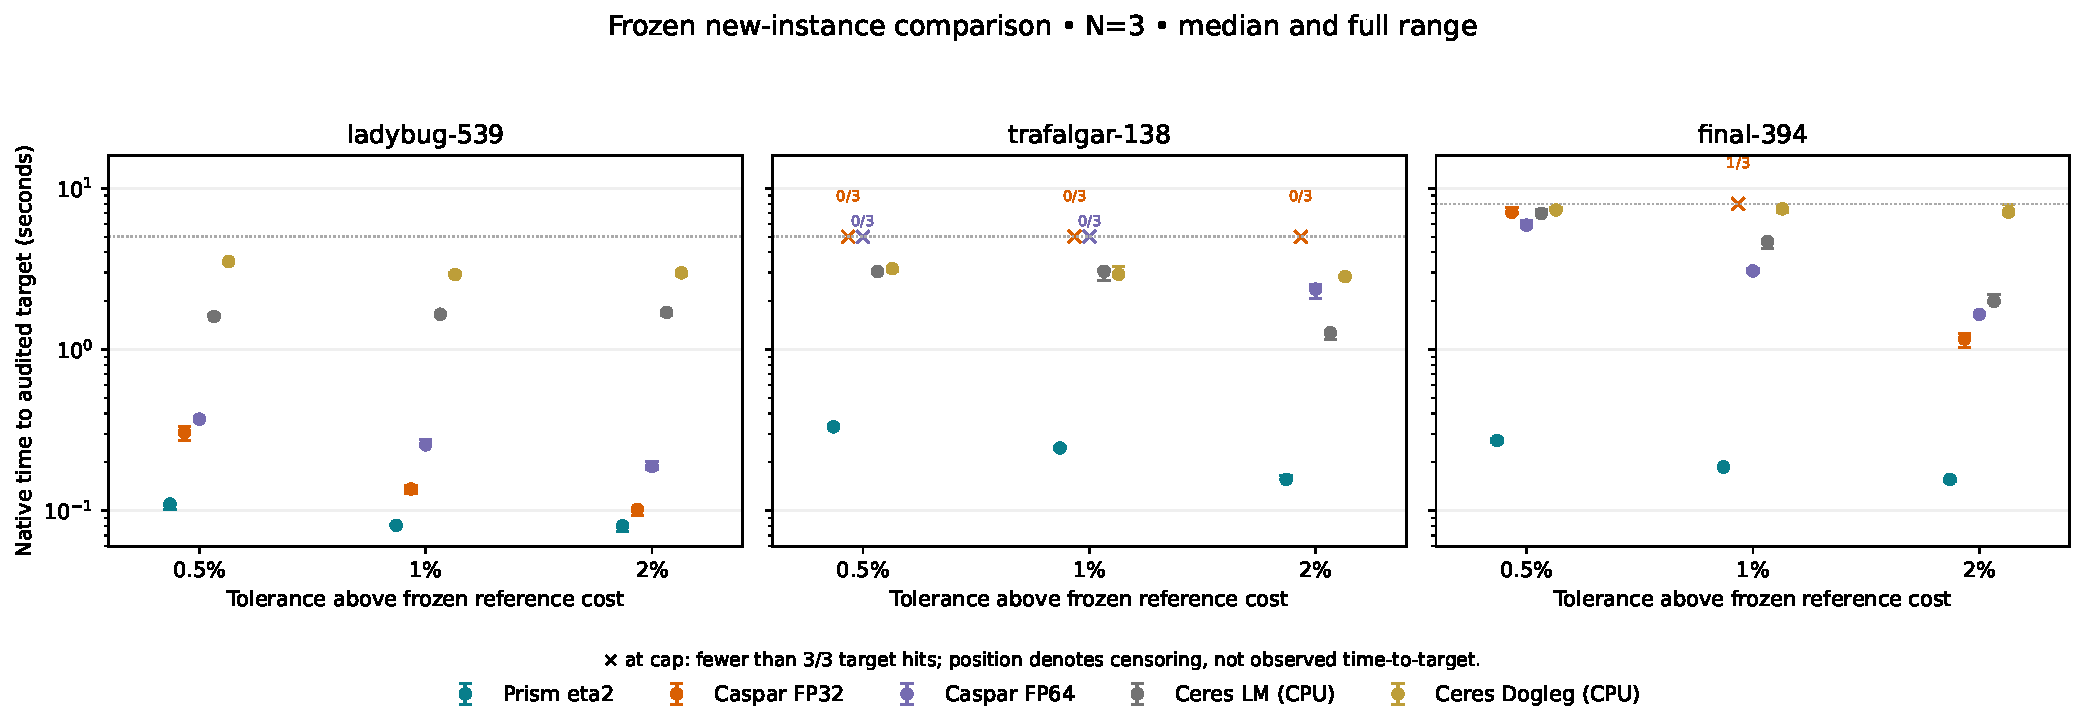
\includegraphics[width=0.88\textwidth]{frozen_new_instances_time_to_target.pdf}
\caption{Frozen time-to-target comparison across three target tolerances on three previously unmeasured local BAL instances.  Missing bars denote target misses rather than zero time.}
\label{fig:newinstances}
\end{figure}

\subsection{Largest BAL problem}

Final-13682 contains 13,682 cameras, 4,456,117 points, and 28,987,644 observations.  At the registered target $27{,}591{,}576.557625$, Eta2 reaches the target after four accepted outer steps, 19 Schur products, and zero nonlinear rejects.  Table~\ref{tab:largest} reports the same-host comparison.

\begin{table}[ht]
\centering
\small
\caption{Final-13682 time to the identical primary target.}
\label{tab:largest}
\begin{tabular}{@{}lcccc@{}}
\toprule
Method & Hits & Median seconds & Range & Audited terminal cost\\
\midrule
Prism Eta2 & 5/5 & \textbf{3.2386} & [3.2375,3.2589] & 27,422,876\\
Prior Prism incumbent & 5/5 & 4.2624 & [4.2583,4.2988] & 26,022,218\\
Caspar FP32 & 3/3 & 7.0838 & [6.4205,7.0857] & 27,516,921\\
Caspar FP64 & 3/3 & 14.9734 & [14.9728,14.9736] & 27,580,841\\
\bottomrule
\end{tabular}
\end{table}

Eta2 is $2.187\times$ faster than the measured Caspar FP32 configuration and $4.623\times$ faster than Caspar FP64 at this target.  Terminal costs differ because the methods cross the threshold on discrete outer iterations; the table is a convergence-to-common-quality comparison, not an equal-time or converged-endpoint ranking.  At the tighter historical target $27{,}318{,}392.631312$, Eta2 requires a fifth accepted outer and takes 4.1173 seconds, versus 4.2625 seconds for the prior Prism incumbent.  Caspar did not reach that tighter target in the reported primary-target runs, so no tighter-target Caspar ratio is inferred.

\begin{figure}[ht]
\centering
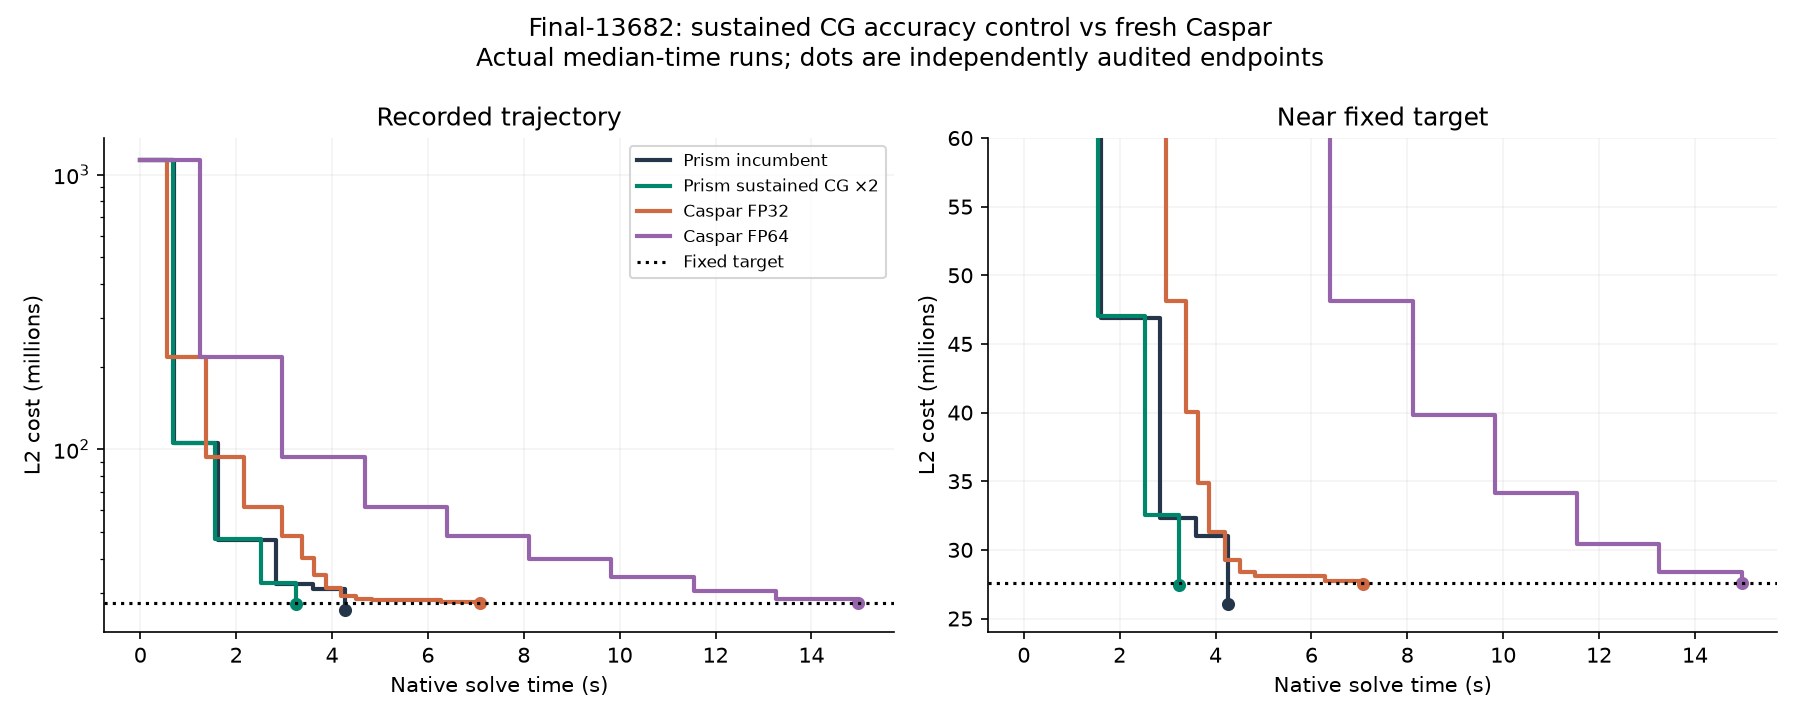
\includegraphics[width=0.96\textwidth]{final13682_sustained_caspar.png}
\caption{Recorded convergence on Final-13682.  Curves are actual representative runs with staircase interpolation between accepted states; table values use native target events and audited terminal states.}
\label{fig:largest}
\end{figure}

\subsection{B6v7 systems candidate}\label{sec:b6v7}

B6v7 changes execution rather than the optimization equations.  Its registered $n_c\ge128$ dispatch uses the deterministic camera-owned reduced-RHS path and dead-diagonal pruning; smaller problems execute the dots-only path.  On the nine-cell practical panel, all 54 runs hit their targets, median products/outers/rejects are unchanged in every cell, and B6v7 is 8.66\% faster in geometric-mean \targettime{} with all nine timing ranges disjoint in its favor.  On Muell it is 4.05\% faster with the same 980 products, 16 outers, and zero rejects.

The stochastic Final-3068 extension used 150 runs per arm.  B6v7 recorded 100/150 hits versus 89/150 for dots-only.  The one-sided 95\% lower bound on the hit-rate difference is $-1.826$ percentage points, passing the registered $-15$-point non-inferiority margin.  Conditional median crossing time falls from 3.669 to 3.269 seconds; all-run mean wall falls from 3.778 to 3.423 seconds.  Superiority of the hit-rate point estimate is not established ($p=0.2317$ in the two-sided Fisher test).  B6v7 therefore remains a separately identified optimized candidate rather than silently replacing the frozen scientific binary.

\subsection{Reliability option}

A separate three-attempt portfolio restarts an unchanged B6v7 solve from the original input after a miss.  It reached 37/38 Final-3068 targets, rescuing 13 of 14 first-attempt misses.  Charged native time was 4.263 seconds median, 5.932 seconds mean, and 10.039 seconds at the 90th percentile.  This crossed its preregistered high-reliability sequential boundary but missed its 3.923-second median-time promotion ceiling.  It is a Pareto option for reliability-sensitive use, applying established algorithm-portfolio logic\cite{GomesSelman2001}, not a faster single-trajectory algorithm or an inner-solver novelty claim.

\subsection{Negative results that delimit the method}

Several strong linear-algebra ideas passed local correctness checks and still failed as native BA changes:
\begin{itemize}
  \item Schur-Jacobi reduced products on some frozen systems but was 1.6\% slower geometrically on the practical panel, 21.3\% slower on Muell, and reduced Final-3068 hits from 4/5 to 1/5.
  \item A dense FP64 Schur/Cholesky path matched the operator but was $1.49$--$2.77\times$ slower on the small Trafalgar cells; on Venice, matrix formation took 56.7 of 60.1 seconds.
  \item A Gram-consistent square-root Schur operator matched the conventional action to $1.80\times10^{-15}$ relative and curvature to $5.91\times10^{-15}$, yet was 1.52\% slower on the panel, 6.55\% slower on Muell, and lost both registered tail tests.
  \item FP32 inner solves with FP64 residual/refinement passed the frozen FP64 residual gate and improved panel wall by 14\%, but changed product counts by $1.07$--$4.40\times$ and moved median endpoints by as much as 0.519\%, violating the registered trajectory-equivalence rule.
  \item A five-shift opening bank was slower and less reliable than Eta2: on Dubrovnik-88, saving one outer still cost 401 versus 53 Schur products; radius clipping could erase the raw amplitude diversity that motivated the menu.
  \item Exact targeted two-view point repair reduced the recorded pathological track costs from 256 and 1,795 to about 0.033, but native Final-3068 reliability was unchanged and Venice's median endpoint worsened 4.15\%.
\end{itemize}
These results are not arguments against the underlying methods in all BA solvers.  They show that, in Eta2, changing the finite inexact direction changes clipping, acceptance, damping history, and basin selection.  A better frozen linear system is not automatically a faster or more reliable nonlinear algorithm.

\section{Interpretation and remaining limitations}

The data support three conclusions.  First, the dominant advantage is convergence speed to useful, common quality.  The Final-13682 gain shrinks at a tighter target, and minor endpoint differences below a percent should not be confused with a convergence-speed regression.  Second, basin selection and stopping create heavy-tail behavior on a subset of scenes, especially Final-3068 and Venice-52.  Large cohorts and explicit hit rates are required there; $N=3$ is adequate only for stable timing cells.  Third, the practical Eta2 speed result comes from a single-shift inexact solver.  The multi-shift design remains a separate research line and cannot be credited for these numbers.

The evidence remains bounded by the following limitations:
\begin{itemize}
  \item Most comparisons use one RTX 2000 Ada host.  Ceres is an eight-thread CPU reference; Caspar is a pinned standalone generated backend, not a complete COLMAP pipeline.
  \item Native solver time excludes text parsing, export, and audit.  Caspar graph setup is also excluded and reported separately.  Final-13682 end-to-end ingestion is dominated by the large text input.
  \item Fixed anchors are bounded calibration endpoints, not certificates of the global optimum.  A target hit demonstrates crossing a registered quality level.
  \item BAL scene families are correlated.  Repeated executions quantify run variability on fixed inputs and do not alone establish generalization to all reconstruction domains.
  \item The exact-policy novelty of the point safeguard and the priority of the mixed-storage recovery combination require a broader prior-art and patent search before a formal novelty claim.
\end{itemize}

\section{Conclusion}

Prism--Eta2 is best described as a safeguarded, matrix-free, inexact GPU LM implementation whose outer policy treats linear work as provisional and validates the actual nonlinear candidate.  Its measured strength is rapid convergence to registered useful quality: it is fastest among the measured configurations on a frozen nine-cell panel and is $2.19\times$ and $4.62\times$ faster than the tested Caspar FP32 and FP64 configurations, respectively, on the largest BAL scene at the common primary target.  The most defensible novelty lies in the combination of nonlinear candidate handling, BA-specific separable rescue, diagnosed mixed-storage Schur recovery, and evidence showing that linear-system improvements can fail through nonlinear trajectory coupling.  B6v7 adds a separate, measurable systems improvement.  A claim of a new general trust-region method, a multi-shift win, an RL contribution, or universal solver supremacy would exceed the present evidence.

\begin{thebibliography}{99}
\small

\bibitem{Agarwal2010}
S. Agarwal, N. Snavely, S. Seitz, and R. Szeliski,
``Bundle Adjustment in the Large,''
\emph{European Conference on Computer Vision}, 2010.
\href{https://grail.cs.washington.edu/projects/bal/bal.pdf}{Preprint}.

\bibitem{Triggs2000}
B. Triggs, P. McLauchlan, R. Hartley, and A. Fitzgibbon,
``Bundle Adjustment---A Modern Synthesis,''
\emph{Vision Algorithms: Theory and Practice}, LNCS 1883, 2000.
\href{https://www.cs.jhu.edu/~misha/ReadingSeminar/Papers/Triggs00.pdf}{Preprint}.

\bibitem{EisenstatWalker1996}
S. Eisenstat and H. Walker,
``Choosing the Forcing Terms in an Inexact Newton Method,''
\emph{SIAM Journal on Scientific Computing}, 17(1), 1996.
\href{https://users.wpi.edu/~walker/Papers/forcing_terms,SISC_17,1996,16-32.pdf}{Author copy}.

\bibitem{Demmel2021}
N. Demmel, C. Sommer, D. Cremers, and V. Usenko,
``Square Root Bundle Adjustment for Large-Scale Reconstruction,''
\emph{IEEE/CVF Conference on Computer Vision and Pattern Recognition}, 2021.
\href{https://www.usenko.net/pdf/demmel2021rootba.pdf}{Author copy}.

\bibitem{Jeong2012}
Y. Jeong, D. Nist\'er, D. Steedly, R. Szeliski, and I.-S. Kweon,
``Pushing the Envelope of Modern Methods for Bundle Adjustment,''
\emph{IEEE Transactions on Pattern Analysis and Machine Intelligence}, 34(8), 2012.
\href{https://szeliski.org/papers/Jeong_BundleAdjustment_CVPR10.pdf}{Conference version}.

\bibitem{Ceres}
S. Agarwal, K. Mierle, and the Ceres Solver Team,
``Ceres Solver,'' version 2.2 documentation and source.
\href{https://ceres-solver.readthedocs.io/latest/nnls_solving.html}{Documentation}.

\bibitem{Caspar2026}
E. Martens, A. Miller, M. Varnum, and A. Stahl,
``Caspar: CUDA Accelerator for Symbolic Programming with Adaptive Reordering,''
arXiv:2605.30583, accepted at ICRA 2026.
\href{https://arxiv.org/abs/2605.30583}{arXiv record}.

\bibitem{GomesSelman2001}
C. Gomes and B. Selman,
``Algorithm Portfolios,''
\emph{Artificial Intelligence}, 126(1--2), 2001.
\href{https://www.cs.cornell.edu/selman/papers/pdf/01.aij.portfolios.pdf}{Author copy}.

\bibitem{Conn2000}
A. Conn, N. Gould, and P. Toint,
\emph{Trust-Region Methods}, SIAM, 2000.

\end{thebibliography}

\appendix
\section{Frozen Eta2 flags}

The principal enabled configuration is reproduced below for identity rather than as a recommendation that every flag is individually beneficial:
\begin{verbatim}
--algo mfree_shifted_cg --dof9 --zero_k2 --lam0 0.1 --max_iter 600
OCA_ATTR_RADIUS=1          OCA_ATTR_RESCUE=1
OCA_ATTR_STRICT=1          OCA_BACKTRACK_REARM=1
OCA_CAMERA_TR=0            OCA_CLASSICAL_LM=1
OCA_COMPACT_FRAGMENTS=2    OCA_DEMAND_MENU=0
OCA_DIAG_NORM=1            OCA_FORCE_UNSHARED=1
OCA_FTOL=1e-5              OCA_FTOL_K=8
OCA_MULTI_RHS=1            OCA_NSHIFTS=1
OCA_PCG=1                  OCA_POINT_SAFEGUARD=1
OCA_RETRY_CACHE=1          OCA_RHO_LAMBDA=1
OCA_RHO_SHIFT=1            OCA_SCHUR_NUMERIC_GUARD=1
OCA_RLA_FIXED_ETA=2
\end{verbatim}

\section{Evidence map}

The claims in this report map to the following repository records:
\begin{itemize}
  \item Formulation and contribution boundary: \path{theory_and_novelty.md}.
  \item Six-scene Eta2 gate and Final-13682 comparison: \path{rl_sustained_results.md}.
  \item Frozen three-instance external baselines: \path{speed_novelty_results.md}.
  \item Numerical recovery controls: \path{schur_recovery_results.md}.
  \item B6v7 performance and non-inferiority: \path{../../eta2_wave5/B6V7_RESULTS.md} and \path{../../eta2_wave5/B6V7_EXTENSION_RESULTS.md}.
  \item Restart portfolio: \path{../../eta2_wave6/D21_RESTART_PORTFOLIO_RESULTS.md}.
\end{itemize}

\end{document}
